\documentclass[a4paper]{article}


\usepackage[T1]{fontenc}
%\usepackage[french]{babel}
\usepackage{ProfLycee}
\useproflyclib{ecritures}
\usepackage{math-vh}
\usepackage{eurosym}
\usepackage{xspace}
\usepackage{tabularx}
\usepackage[table]{xcolor}


\renewcommand\euro{\officialeuro\xspace}
% *** Réglage des headers ***
\fancyhead[L]{2GT --- Lycée Victor Hugo}
\fancyhead[R]{Année 2024-2025}
% *** Réglage des headers ***


\begin{document}

\begin{center}
  {\scshape\LARGE Révisions Thème 1 - Repérage\par}
  \vspace{0.5cm}
\end{center}



\begin{methode*}[sidebyside, righthand width=2.2cm,segmentation code={}, sidebyside align=top]{Calculer les coordonnées du milieu d'un segment $\longrightarrow$ Exercices 1, 3, 4, 5, 6}{}
  \begin{tabular}{cc}
    \begin{minipage}{8cm}
      
  Soit le segment $[AB]$ avec $A(2; 3)$ et $B(6; 7)$.

  Les coordonnées du milieu $M$ sont données par:
  $$
  M\left(\dfrac{x_A + x_B}{2}; \dfrac{y_A + y_B}{2}\right)
  $$

  En appliquant ces formules, on obtient :
  $$
  M\left(\dfrac{2 + 6}{2}; \dfrac{3 + 7}{2}\right) \text{ soit } M(4; 5)
  $$
    \end{minipage}&

  \begin{minipage}{6cm}
    
  \begin{center}
    \begin{tikzpicture}[scale=0.7,x=0.8cm,y=0.6cm, %unités
      xmin=-1,xmax=7,xgrille=1,xgrilles=1, %axe Ox 
      ymin=-1,ymax=8,ygrille=1,ygrilles=1] %axe Oy
      
      \FenetreSimpleTikz%
      <Police=\small>{1,2,...,6}%
      <Police=\small>{1,2,...,7} %repère
  
      \draw[thick] (2,3) -- (6,7);
      \filldraw[blue] (2,3) circle (2pt) node[below] {$A(2; 3)$};
      \filldraw[blue] (6,7) circle (2pt) node[left] {$B(6; 7)$};
      \filldraw[red] (4,5) circle (2pt) node[below right] {$M(4; 5)$};
      \draw[dashed] (4,0) -- (4,5);
      \draw[dashed] (0,5) -- (4,5);
  \end{tikzpicture}
    \end{center}
  \end{minipage} 
  \\
  \end{tabular}

  \tcblower
  \vspace{2cm}
  \SimpleQRCode{https://www.youtube.com/watch?v=YTQCtSvxAmM}{1.2cm}

\end{methode*}


\begin{methode*}[sidebyside, righthand width=2.2cm,segmentation code={}, sidebyside align=bottom]{Calculer la longueur d'un segment $\longrightarrow$ Exercices 1, 2, 5, 6}{}

  Soit le segment $[AB]$ avec $A(1; 2)$ et $B(4; 6)$.

  La longueur du segment $[AB]$ est donnée par la formule suivante :
  $$
  AB = \sqrt{(x_B - x_A)^2 + (y_B - y_A)^2}
  $$

  En appliquant cette formule, on obtient :
  $$
  AB = \sqrt{(4 - 1)^2 + (6 - 2)^2} = \sqrt{3^2 + 4^2} = \sqrt{9 + 16} = \sqrt{25} = 5
  $$

  \tcblower
  
  \SimpleQRCode{https://www.youtube.com/watch?v=pP8ebg8W9o8}{1.2cm}


\end{methode*}


\begin{methode*}[sidebyside, righthand width=2.2cm,segmentation code={}, sidebyside align=top]{Calculer les coordonnées du symétrique d'un point $\longrightarrow$ Exercices 1, 4, 6}{}

  \begin{tabular}{cc}
    \begin{minipage}{8cm}

      Soit le point $A(2; 3)$ et le point $B(6; 7)$. Calculons les coordonnées du symétrique $C(x_C;y_C)$ de $A$ par rapport au point $B$.

      $B$ est le milieu de $[AC]$, donc on doit résoudre le système suivant :
      
      $\begin{dcases}
        x_B = \dfrac{x_A + x_C}{2} \\
        y_B = \dfrac{y_A + y_C}{2}
      \end{dcases} \iff \begin{dcases}
        6 = \dfrac{2 + x_C}{2} \\
        7 = \dfrac{3 + y_C}{2}
      \end{dcases}$

      $\iff \begin{dcases}
        12 = 2 + x_C \\
        14 = 3 + y_C
      \end{dcases}
      \iff \begin{dcases}
        x_C = 10 \\
        y_C = 11
      \end{dcases}$
      
      Le point $C$ a donc pour coordonnées $(10; 11)$.
    \end{minipage}&

  \begin{minipage}{6cm}
    
  \begin{center}
    \begin{tikzpicture}[scale=0.5,x=0.8cm,y=0.6cm, %unités
      xmin=-1,xmax=12,xgrille=1,xgrilles=1, %axe Ox 
      ymin=-1,ymax=12,ygrille=1,ygrilles=1] %axe Oy
      
      \FenetreSimpleTikz%
      <Police=\small>{1,2,...,11}%
      <Police=\small>{1,2,...,11} %repère
  
      \draw[thick] (2,3) -- (6,7) -- (10,11);
      \filldraw[blue] (2,3) circle (2pt) node[below right] {$A(2; 3)$};
      \filldraw[blue] (6,7) circle (2pt) node[below right] {$B(6; 7)$};
      \filldraw[red] (10,11) circle (2pt) node[left] {$C(10; 11)$};
      \draw[dashed] (6,0) -- (6,7);
      \draw[dashed] (0,7) -- (6,7);
  
       
    \end{tikzpicture}
    \end{center}
  \end{minipage}
  \\
  \end{tabular}
  \tcblower
  
  \vspace{2.5cm}
  \SimpleQRCode{https://www.youtube.com/watch?v=XNlkPc1P3_o}{1.2cm}


\end{methode*}

\setcounter{exercice}{0}

\begin{exercice}{}{}
  $~$
  \begin{center}

    \begin{tabular}{cc}
      \begin{minipage}{9cm}
        On considère le repère ci-contre:
    
    
    
        \begin{enumerate}
            \item Donner les coordonnées des points $A$, $B$, $C$, $D$.
            \item Le triangle $ACD$ est-il isocèle en $C$?
            \item Placer dans ce repère les points $E(3;0)$, $F(-2;-1)$ et $G(0;4)$.
            \item Quelles sont les coordonnées des points $P$ et $Q$, milieux respectifs de $[AB]$ et $[DE]$? Placer $P$ et $Q$ sur le repère.
            \item Soit $K(3;-4)$. Calculer les coordonnées de $G$ pour que $K$ soit le milieu de $[CG]$.
        \end{enumerate}
         
      \end{minipage}
      &
    
      \begin{minipage}{8cm}
        \begin{tikzpicture}[x=0.7cm,y=0.7cm, %unités
            xmin=-5,xmax=5,xgrille=1,xgrilles=1, %axe Ox 
            ymin=-5,ymax=5,ygrille=1,ygrilles=1] %axe Oy
            
            \FenetreSimpleTikz%
            <Police=\small>{-5,-4,-3,-2,-1,1,2,...,4}%
            <Police=\small>{-5,-4,-3,-2,-1,1,2,...,4} %repère
        
            \draw (1,2) node[cross=2pt,blue]{};
            \node[above right, blue] at (1,2){$A$};
        
            \draw (-1,1) node[cross=2pt,blue]{};
            \node[above left, blue] at (-1,1){$B$};
        
            \draw (2,-2) node[cross=2pt,blue]{};
            \node[below right, blue] at (2,-2){$C$};
        
            \draw (-2,0) node[cross=2pt,blue]{};
            \node[above left, blue] at (-2,0){$D$};
        \end{tikzpicture}
      \end{minipage}
    
    \end{tabular}
  \end{center}
\end{exercice}

\medskip

\begin{exercice}{}{}
    Dans un repère orthonormé, on donne $A(-2; 3)$, $B(3;2)$ et $C(0;0)$.

    \begin{enumerate}
        \item Calculer les distances $AB$, $AC$ et $BC$.
        \item Le triangle $ABC$ est-il rectangle?
    \end{enumerate}
\end{exercice}
\medskip

\begin{exercice}{}{}
Dans un repère orthonormé, on donne $A(-3;\sqrt{2})$ et $B(2;-\sqrt{2})$.

Déterminer les coordonnées du milieu $I$ de $[AB]$.
    
\end{exercice}

\medskip
\begin{exercice}{}{}
    Dans un repère du plan, on considère les points $E(3;4)$, $F(6;6)$ et $G(4;-1)$.

    Calculer les coordonnées du point $H$ tel que $EFGH$ soit un parallélogramme.
\end{exercice}

\medskip
\begin{exercice}{}{}
Dans un repère orthonormé du plan, on considère les points $A(4;1)$, $B(0;4)$ et $C(-6;-4)$.
\begin{enumerate}
    \item Calculer $AB$, $AC$ et $BC$.
    \item En déduire que le triangle $ABC$ est rectangle.
    \item Trouver les coordonnées du centre du cercle circonscrit à ce triangle. Quel est son rayon?
\end{enumerate}
\end{exercice}

\medskip
\begin{exercice}{}{}
     Dans le plan muni d'un repère orthonormé $(0;I,J)$, on considère les points $A(-3;0)$, $B(2;1)$, $C(4;3)$ et $D(-1;2)$.

     \begin{enumerate}
         \item Placer les points $A$, $B$, $C$ et $D$.
         \item Démontrer que les segments $[AC]$ et $[BD]$ ont le même milieu $K$.
         \item Montrer que le triangle $OBD$ est rectangle isocèle.
         \item On considère le point $E$ du plan tel que $BODE$ soit un parallélogramme. Quelles sont les coordonnées de $E$?
         \item Calculer $AE$.
     \end{enumerate}
\end{exercice}


\pagebreak



\begin{center}
    {\scshape\LARGE Révisions Thème 2 - Vecteurs\par}
    \vspace{0.5cm}
  \end{center}
  
  \setcounter{exercice}{0}

  \begin{methode*}[sidebyside, righthand width=2.2cm,segmentation code={}]{Construire un point à partir d'une somme de vecteurs $\longrightarrow$ Exercices 3, 4 et 5}{}
   
   \begin{tabular}{cc}
    \begin{minipage}{8cm}
      
    Soit $ABC$ un triangle. Placer le point $D$ tel que $\Vecteur{BD}=2\Vecteur{AB}+\Vecteur{CB}$.
 
    \begin{enumerate}
      \item On trace le vecteur $2\Vecteur{AB}$ à partir du point $B$.
      \item On trace le vecteur $\Vecteur{CB}$ à la suite.
      \item On place le point $D$ tel que $\Vecteur{BD}=2\Vecteur{AB}+\Vecteur{CB}$.
    \end{enumerate}
    \end{minipage} &

    \begin{minipage}{6cm}
      
    \begin{center}
      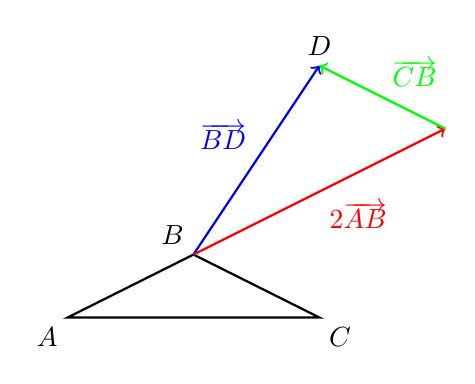
\begin{tikzpicture}[scale=0.8]
        % Points
        \coordinate (A) at (0,0);
        \coordinate (B) at (2,1);
        \coordinate (C) at (4,0);
        \coordinate (D) at (4,4);

        % Triangle ABC
        \draw[thick] (A) -- (B) -- (C) -- cycle;

        % Vecteur BD
        \draw[thick,->,blue] (B) -- (D) node[midway, above left] {$\overrightarrow{BD}$};

        % Vecteur 2AB
        \draw[thick,->,red] (B) -- ++(4,2) node[midway, below right] {$2\overrightarrow{AB}$};

        % Vecteur CB
        \draw[thick,->,green] (6,3) -- ++(-2,1) node[midway, above right] {$\overrightarrow{CB}$};

        % Points labels
        \node[below left] at (A) {$A$};
        \node[above left] at (B) {$B$};
        \node[below right] at (C) {$C$};
        \node[above] at (D) {$D$};
      \end{tikzpicture}
    \end{center}
    \end{minipage}
   \end{tabular}
  

        \tcblower
        \vspace{2cm}
    \SimpleQRCode{https://www.youtube.com/watch?v=nzABUzFM6p8}{1.2cm}
  \end{methode*}

  \begin{methode*}[sidebyside, righthand width=2.2cm,segmentation code={}]{Appliquer la relation de Chasles $\longrightarrow$ Exercices 4 et 5}{}
  
    Soient les points $A$, $B$ et $C$. La relation de Chasles s'écrit :
    $\overrightarrow{A\underline{B}} + \overrightarrow{\underline{B}C} = \overrightarrow{AC}$

    \begin{center}
      \begin{tikzpicture}
        % Points
        \coordinate (A) at (0,0);
        \coordinate (B) at (2,1);
        \coordinate (C) at (4,0);

        % Vecteurs
        \draw[thick,-{Stealth[scale=1]}] (A) -- (B) node[midway, above left] {$\overrightarrow{AB}$};
        \draw[thick,-{Stealth[scale=1]}] (B) -- (C) node[midway, above right] {$\overrightarrow{BC}$};
        \draw[thick,-{Stealth[scale=1]},red] (A) -- (C) node[midway, below] {$\overrightarrow{AC}$};

        % Points labels
        \node[below left] at (A) {$A$};
        \node[above] at (B) {$B$};
        \node[below right] at (C) {$C$};
      \end{tikzpicture}
    \end{center}
    \tcblower
    \vspace{2cm}
\SimpleQRCode{https://www.youtube.com/watch?v=fbVrdYiY0qc}{1.2cm}
  \end{methode*}
  
  \medskip
  
  \begin{exercice}{}{}
  
  A partir de la figure, citer un vecteur:

  \begin{center}
  \begin{tabular}{cc}
    \begin{minipage}{7cm}
  
  
      \begin{enumerate}
        \item de même direction et de même sens que $\overrightarrow{AB}$.
        \item de même direction que $\overrightarrow{CD}$ mais de sens contraire.
        \item dont la norme est égale à $\lVert \overrightarrow{CD} \rVert$.
      \end{enumerate}
     
    \end{minipage}&
    \begin{minipage}{10cm}
      \begin{center}
        \begin{tikzpicture}[scale=0.8]

          % Grille
          \draw[gray, thin] (0,0) grid (11,9);
          
          % Vecteurs
          \draw[-{Stealth[scale=1]}, blue, very thick] (2,5) -- (4,8) node[midway, above left] {$\vec{v}$};
          \draw[-{Stealth[scale=1]}, violet,very thick] (5,5) -- (5,7) node[midway, right] {$\vec{w}$};
          \draw[-{Stealth[scale=1]}, orange,very thick] (1,3) -- (2,3) node[midway, below] {$\vec{u}$};
          \draw[-{Stealth[scale=1]}, red,very thick] (6,6) -- (7,7) node[midway, above left] {$\vec{r}$};
          \draw[-{Stealth[scale=1]}, gray,very thick] (9,8) -- (7,3) node[midway, above left] {$\vec{s}$};
          \draw[-{Stealth[scale=1]}, ForestGreen,very thick] (9,8) -- (8,8) node[midway, above] {$\vec{t}$};
          \draw[-{Stealth[scale=1]}, cyan,very thick] (10,2) -- (9,1) node[midway, below right] {$\vec{p}$};
          \draw[-{Stealth[scale=1]}, brown,very thick] (10,5) -- (10,4) node[midway, right] {$\vec{m}$};
          
          % Points
          \node[above] at (4,4) {A};
          \filldraw (4,4) circle (2pt);
          \node[below] at (2,1) {B};
          \filldraw (2,1) circle (2pt);
          \node[below] at (4,1) {C};
          \filldraw (4,1) circle (2pt);
          \node[below] at (5,2) {D};
          \filldraw (5,2) circle (2pt);
          
          \end{tikzpicture}
        \end{center}
    \end{minipage}\\
  \end{tabular}
  \end{center}
  \begin{center}
 

    
  \end{center}
  \end{exercice}
  
  \begin{exercice}{}{}
    On considère ci-dessous l'hexagone régulier $ABCDEF$ de centre $G$.

    \begin{center}
    \begin{tabular}{cc}
      \begin{minipage}{7cm}
  
        \begin{enumerate}
          \item Citer un vecteur qui a même direction que le vecteur $\overrightarrow{FG}$ mais pas le même sens.
          \item Citer le représentant d'origine $G$ du vecteur $\overrightarrow{BC}$.
          \item Citer deux vecteurs égaux au vecteur $\overrightarrow{AF}$.
        \end{enumerate}
      \end{minipage}&
      \begin{minipage}{10cm}
        \begin{center}
          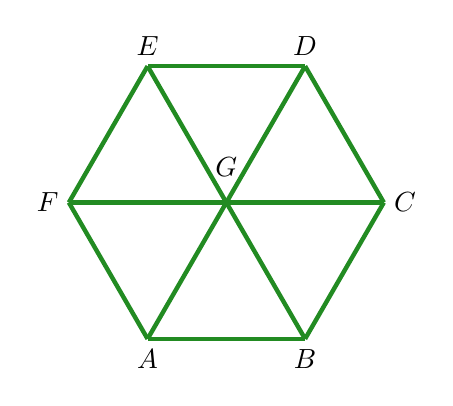
\begin{tikzpicture}[scale=1]
            \draw[ForestGreen, ultra thick] (60*0:2cm) -- (60*0+60:2cm) node[black, above, thick ] {$D$};
            \draw[ForestGreen, ultra thick] (60*1:2cm) -- (60*1+60:2cm) node[black, above, thick ] {$E$};
            \draw[ForestGreen, ultra thick] (60*2:2cm) -- (60*2+60:2cm) node[black, left, thick ] {$F$};
            \draw[ForestGreen, ultra thick] (60*3:2cm) -- (60*3+60:2cm) node[black, below, thick ] {$A$};
            \draw[ForestGreen, ultra thick] (60*4:2cm) -- (60*4+60:2cm) node[black, below, thick ] {$B$};
            \draw[ForestGreen, ultra thick] (60*5:2cm) -- (60*5+60:2cm) node[black, right, thick ] {$C$};
  
  
            \draw[ForestGreen, ultra thick] (60*2+60:2cm) -- (60*5+60:2cm) node[black, left, thick ] {};
            \draw[ForestGreen, ultra thick] (60*3+60:2cm) -- (60*0+60:2cm) node[black, left, thick ] {};
            \draw[ForestGreen, ultra thick] (60*4+60:2cm) -- (60*1+60:2cm) node[black, left, thick ] {};
  
            \draw (0,0.2)node[black, above, thick ] {$G$};
          \end{tikzpicture}
        \end{center}
      \end{minipage}
  
    \end{tabular}
    \end{center}  
  
  \end{exercice}
  
  \pagebreak
  
  \begin{exercice}{}{}
    La figure ci-dessous est constituée de neuf triangles équilatéraux.
  
    \begin{tabular}{cc}
      \begin{minipage}{7cm}
  
        \begin{center}
          \includegraphics[width=6cm]{img/exo3.png}
          \end{center}
      \end{minipage}&
      \begin{minipage}{10cm}
  
        En utilisant les points de la figure, déterminer:
        \begin{enumerate}
          \item un vecteur égal à $\overrightarrow{IJ}+2\overrightarrow{JN}$.
          \item un vecteur égal à $2\overrightarrow{IO}+2\overrightarrow{QN}$.
          \item un vecteur égal à $\dfrac{2}{3}\overrightarrow{IL}+\dfrac{1}{2}\overrightarrow{OR}$.
          \item un vecteur égal à $-\dfrac{1}{3}\overrightarrow{RL}-\dfrac{1}{2}\overrightarrow{OR}$.
        \end{enumerate}
      \end{minipage}\\
    \end{tabular}
  \end{exercice}
  
  \medskip
  \begin{exercice}{}{}
  
      Soit un rectangle $ABCD$ tel que $AC = 5$. Les points $M$et $N$ sont tels que:
   
   $$\begin{dcases}
    \overrightarrow{AM}=\dfrac{1}{5}\overrightarrow{AC}\\
    \overrightarrow{CN}=\dfrac{1}{5}\overrightarrow{CA}
   \end{dcases}$$
   \begin{enumerate}
       \item Réaliser une figure
       \item Démontrer que $\overrightarrow{MB}=\overrightarrow{DN}$.
       \item Que peut-on en conclure?
   \end{enumerate}
  
      
  \end{exercice}
  \medskip
  
  \begin{exercice}{}{}
      Soit un triangle quelconque $ABC$ et les points $D$ et $E$ tels que:
      $$\begin{dcases}
        \overrightarrow{AD}=\dfrac{1}{4}\overrightarrow{AC} \\
        \overrightarrow{AE}=\dfrac{1}{4}\overrightarrow{AB}
      \end{dcases}$$
  \begin{enumerate}
      \item Justifier que  $\overrightarrow{DE}=\dfrac{1}{4}\overrightarrow{CB}$.
      \item Quelle est la nature du quadrilatère $DEBC$?
  \end{enumerate}  
  
      
  \end{exercice}
  
  
  \pagebreak
  

  

\begin{center}
    {\scshape\LARGE Révisions Thème 3 - Information chiffrée\par}
    \vspace{0.5cm}
  \end{center}
  

  \begin{methode*}[sidebyside, righthand width=2.2cm,segmentation code={}]{Calculer une évolution $\longrightarrow$ Exercices 1, 3, 4, 7 et 8}{}
     Un article vendu $50$\euro subit une hausse de $20\%$. Quel est son nouveau prix?

     \begin{itemize}
      \item On calcule le coefficient multiplicateur correspondant à la hausse: $1 + \frac{20}{100} = 1,2$.
      \item On multiplie le prix initial par ce coefficient: $50$\euro$ \times 1,2 = 60$\euro.
     \end{itemize}
    \tcblower
    %\vspace{2cm}
    \SimpleQRCode{https://www.youtube.com/watch?v=UVXFEDUnSjI}{1.2cm}
  \end{methode*}
  

  \begin{methode*}[sidebyside, righthand width=2.2cm,segmentation code={}]{Calculer des taux d'évolutions successifs $\longrightarrow$ Exercices 3, 7 et 8}{}
    Un article subit une hausse de $30\%$ puis une baisse de $10\%$. Quel est le taux d'évolution global?

    \begin{itemize}
     \item Coefficient multiplicateur correspondant à la première évolution: $1 + \frac{30}{100} = 1,3$.
     \item Coefficient multiplicateur correspondant à la seconde évolution: $1 - \frac{10}{100} = 0,9$.
     \item On multiplie ces deux coefficients pour obtenir le coefficient global: $1,3 \times 0,9 = 1,17$.
     
     Le taux d'évolution global est donc de $17\%$.
    \end{itemize}
   \tcblower
   \vspace{1.1cm}
   \SimpleQRCode{https://www.youtube.com/watch?v=qOg2eXd8Hv0}{1.2cm}
 \end{methode*}

 \begin{methode*}[sidebyside, righthand width=2.2cm,segmentation code={}]{Calculer un taux d'évolution réciproque $\longrightarrow$ Exercices 4, 7 et 8}{}
    Un article subit une hausse de $40\%$. Quel est le taux de réduction à appliquer pour retrouver le prix initial?
    
    \begin{itemize}
      \item Le coefficient multiplicateur correspondant à la hausse est: $1 + \frac{40}{100} = 1,4$.
      \item Le coefficient multiplicateur réciproque est : $\frac{1}{1,4} \approx 0,7143$.
      \item Le taux de réduction est donc environ: $1 - 0,7143 = 0,2857 = 28,57\%$.
    \end{itemize}
   \tcblower
   \vspace{1.1cm}
   \SimpleQRCode{https://www.youtube.com/watch?v=NiCxHYkpNiM}{1.2cm}
 \end{methode*}

  
  \medskip
  \setcounter{exercice}{0}
  
  \begin{exercice}{}{}
  Compléter le tableau suivant:
  
  \begin{center}
    \begin{tabular}{|c|c|c|c|}
      \hline 
      \cellcolor{Blue!15!white}\textbf{Prix initial} & \cellcolor{Blue!15!white}\textbf{Prix final} & \cellcolor{Blue!15!white}\textbf{\% de variation} & \cellcolor{Blue!15!white}\textbf{Coefficient multiplicateur} \\
      \hline
      $17$\euro & & $+14\%$ & \\
      \hline
      & $120$\euro&  $-20\%$& \\
      \hline
      $544$\euro& & & $0,915$\\
      \hline
      & $11$\euro& & $1,237$\\
      \hline
      $4$\euro& & $+7,3\%$& \\
      \hline
      $123$\euro& $132$\euro & & \\
      \hline
      $11$\euro& $9,50$\euro& & \\
      \hline
    \end{tabular}
  \end{center}
      
  \end{exercice}
  
  \medskip
  \begin{exercice}{}{}
  
    $200$ salariés d'une entreprise sont répartis suivant trois catégories: ouvriers, techniciens et cadres. L'entreprise 
    compte $120$ femmes selon la répartition suivante:
    \begin{center}
      \begin{tabular}{C{3cm}|*{3}{C{2cm}|}}
        \hhline{~---}
          &\cellcolor{Blue!15!white} Femmes	&\cellcolor{Blue!15!white} Hommes & \cellcolor{Blue!15!white} Total	\\ \hline
        \multicolumn{1}{|C{3cm}|}{\cellcolor{Blue!15!white} Ouvriers}				&78			&			& 114\\ \hline
        \multicolumn{1}{|C{3cm}|}{\cellcolor{Blue!15!white} Techniciens}				&  		& 36		& 54 \\ \hline
        \multicolumn{1}{|C{3cm}|}{\cellcolor{Blue!15!white} Cadres}				& 24 		& 		&  \\ \hline
        \multicolumn{1}{|C{3cm}|}{\cellcolor{Blue!15!white} Total} 					&			&		80	&200 \\ \hline
      \end{tabular}
  
    \end{center}
  
    \begin{enumerate}
      \item Compléter le tableau.
      \item Quel est le pourcentage :
      \begin{enumerate}
        \item d'hommes parmi les salariés de l'entreprise?
        \item de cadres parmi les salariés de l'entreprise?
        \item de femmes parmi les ouvriers ?
        \item de techniciens parmi les femmes ?
      \end{enumerate}
    \end{enumerate}
  \end{exercice}
  
  \medskip
  
  \begin{exercice}{}{}
    Dans chaque cas, donner la réponse exacte en justifiant.
    \begin{enumerate}
      \item Dans un lycée, il y a $1380$ élèves, dont $45\%$ de filles. Le nombre de garçons est:
    
      \begin{tabularx}{\linewidth}{*{4}{>{\bfseries\arraybackslash}p{5mm}@{}X}}
        a.& $621$ &
        b.& $704$ &
        c.& $759$ &
        d.& $828$\\
      \end{tabularx}
  
  
      \item Les trois quarts des clients d'un gîte sont étrangers. Parmi ceux-ci, $80\%$ sont satisfaits
      de leur séjour. Le pourcentage de clients étrangers satisfaits est ...
    
      \begin{tabularx}{\linewidth}{*{4}{>{\bfseries\arraybackslash}p{5mm}@{}X}}
        a.& $40\%$ &
        b.& $60\%$ &
        c.& $75\%$ &
        d.& $80\%$\\
      \end{tabularx}
  
  
      \item Diminuer une quantité de $15\%$, c'est la...
    
      \begin{tabularx}{\linewidth}{*{4}{>{\bfseries\arraybackslash}p{5mm}@{}X}}
        a.& multiplier par $0,15$ &
        b.& diviser par $0,15$ &
        c.& multiplier par $1,15$ &
        d.& diviser par $1,15$\\
      \end{tabularx}
   
      \item Le salaire de Mélissa est passé de $1625$\euro à $1638$\euro. Il a augmenté de ...
    
      \begin{tabularx}{\linewidth}{*{4}{>{\bfseries\arraybackslash}p{5mm}@{}X}}
        a.& $0,8\%$ &
        b.& $0,08\%$ &
        c.& $8\%$ &
        d.& $13\%$\\
      \end{tabularx}
      \pagebreak
   
      \item Une quantité qui a subi une hausse de $10\%$ puis une baisse de $50\%$ a ...
    
      \begin{tabularx}{\linewidth}{*{4}{>{\bfseries\arraybackslash}p{5mm}@{}X}}
        a.& augmenté de $55\%$ &
        b.& baissé de $55\%$ &
        c.& augmenté de $45\%$ &
        d.& baissé de $45\%$\\
      \end{tabularx}
  
   
  
    \end{enumerate}
  \end{exercice}
  
  \medskip
  
  \begin{exercice}{}{}
    Dans chaque cas, donner la ou les bonnes réponses en justifiant.
    \begin{enumerate}
      \item Dans une classe de $32$ élèves, 24 élèves ont un vélo. La proportion des élèves ayant un vélo est
    
      \begin{tabularx}{\linewidth}{*{4}{>{\bfseries\arraybackslash}p{5mm}@{}X}}
        a.& $\dfrac{24}{32}$ &
        b.& $\dfrac{3}{4}$ &
        c.& $0,75$ &
        d.& $75\%$\\
      \end{tabularx}
  
  
      \item On agrandit une longueur $d$ de $20\%$. Elle devient ...
    
      \begin{tabularx}{\linewidth}{*{4}{>{\bfseries\arraybackslash}p{5mm}@{}X}}
        a.& $0,2d$ &
        b.& $1,2d$ &
        c.& $d+\dfrac{20}{100}d$ &
        d.& $20d$\\
      \end{tabularx}
  
  
      \item La vitesse en centre ville est passé de $50 km.h^{-1}$ à $30 km.h^{-1}$. Le taux 
      d'évolution est ...
    
      \begin{tabularx}{\linewidth}{*{4}{>{\bfseries\arraybackslash}p{5mm}@{}X}}
        a.& $\dfrac{30-50}{50}$ &
        b.& $\dfrac{50-30}{30}$ &
        c.& $-0,4$ &
        d.& $-40\%$\\
      \end{tabularx}
   
      \item La population d'une ville a baissé de $4\%$. Pour retrouver sa valeur initiale, elle doit ...
    
      \begin{tabularx}{\linewidth}{*{2}{>{\bfseries\arraybackslash}p{5mm}@{}X}}
        a.& augmenter de $4\%$ &
        b.& être multipliée par $\dfrac{1}{1,04}$ \\
        c.& être divisée par $0,96$ &
        d.& être multipliée par $\dfrac{25}{24}$ \\
      \end{tabularx}
   
  
    \end{enumerate}
  \end{exercice}
  
  \medskip
  
  \begin{exercice}{}{}
  Au sein d'un lycée de $800$ élèves, $276$ lycéens pratiquent du sport dans un club, $12\%$ des lycéens sont inscrits à 
  une fédération sportive scolaire et $9\%$ des lycéens sont inscrits dans un club et à une fédération sportive scolaire.
  \begin{enumerate}
    \item Calculer la proportion, en pourcentage, d'élèves de ce lycée pratiquant du sport dans un club.
    \item Déterminer le nombre d'élèves inscrits à une fédération sportive scolaire.
    \item Déterminer la proportion, en pourcentage, de lycéens pratiquant un sport au sein d'un club ou d'une fédération sportive scolaire.
    \item Déterminer la proportion, en pourcentage, de lycéens ne pratiquant de sport ni au sein d'un club, ni au sein d'une fédération sportive scolaire.
  \end{enumerate}
  \end{exercice}
  
  
  \medskip
  
  \begin{exercice}{}{}
    Dans une grande ville, $78000$ personnes sont inscrites sur les listes électorales.
  
    Lors d'une élection, $57\%$ des personnes inscrites se sont abstenues et $90\%$ des personnes 
    qui ont voté (votants) se sont exprimées (suffrages exprimés).
    
    Le candidat favori est en tête avec exactement $54\%$ des suffrages exprimés.
    \begin{enumerate}
      \item Calculer de deux manières différentes la proportion des suffrages exprimés parmi la totalité des inscrits.
      \item Calculer la proportion, en pourcentage, de bulletins pour le candidat favori parmi les votants, puis parmi les inscrits.
    \end{enumerate}
  \end{exercice}
  
  
  \medskip
  \pagebreak
  \begin{exercice}{}{}
  
    Le tableau ci-dessous donne partiellement la fréquentation du cinéma en France de $2007$ à $2017$, en millions de spectateurs.
  
  
  \begin{center}
    \begin{tabular}{|c|c|c|c|c|c|c|}
      \hline 
      \cellcolor{Blue!15!white}\textbf{Année} &  $2007$ & $2008$ & $2009$ & $2013$ & $2016$ & $2017$\\
      \hline
      \cellcolor{Blue!15!white}\textbf{Spectateurs (en millions)} & $120,9$ & & $201,6$ & & $213,1$ & \\
      \hline
    \end{tabular}
  \end{center}
  
  \begin{enumerate}
    \item Calculer le nombre de spectateurs en $2008$ après une augmentation de $7,7\%$ par rapport à l'année précédente.
    \item Calculer la variation absolue, puis le taux d'évolution (en \%) du nombre de spectateurs de $2007$ à $2009$.
    \item Calculer la fréquentation en $2013$ sachant que la variation relative du nombre de spectateurs de $2013$ à $2016$ est de $0,1002$.
    \item Calculer la fréquentation en $2017$ sachant que le taux d'évolution du nombre de spectateurs de $2016$ à $2017$ est de $-1,8\%$.
  \end{enumerate}
  
  \end{exercice}
  
  
  \medskip
  
  \begin{exercice}{}{}
    \begin{enumerate}
      \item Le prix d'un article subit trois évolutions successives: une hausse de $8\%$, une baisse de $12\%$ et enfin une hausse de $10\%$.
      
      Déterminer le taux d'évolution global (en \%) du prix de l'article.
  
      \item Les ventes d'un article ont baissé de $20\%$ de $2017$ à $2018$.
      Déterminer l'évolution (en \%) des ventes de l'article qu'il faudrait atteindre de $2018$ à $2019$ pour
      revenir à la même quantité qu'en $2017$.
    \end{enumerate}
  \end{exercice}
  
  
  \pagebreak


\begin{center}
    {\scshape\LARGE Révisions Thème 4 - Etude de fonction\par}
    \vspace{0.5cm}
  \end{center}
  
  \setcounter{exercice}{0}
  

  \begin{methode*}[sidebyside, righthand width=2.2cm,segmentation code={}]{Résoudre graphiquement une équation ou une inéquation $\longrightarrow$ Exercices 1, 3}{}
    \begin{center}
      \begin{tabular}{cc}
        \begin{minipage}{8cm}
          Résoudre graphiquement l'inéquation $f(x) \leqslant g(x)$:
          \begin{itemize}
            \item On repère la partie de la courbe $\mathcal{C}_f$ qui est en dessous de la courbe $\mathcal{C}_g$.
            \item On lit les abscisses des points de cette partie de la courbe $\mathcal{C}_f$.
            \item L'ensemble des solutions est $\mathcal{S}=\IntervalleFF{-1}{4}$.
          \end{itemize}
        \end{minipage}&
        \begin{minipage}{7cm}
          \begin{center}
            \begin{tikzpicture}[x=.6cm,y=.4cm,%unités
              xmin=-4,xmax=6,xgrille=1,xgrilles=1, %axe Ox
              ymin=-1,ymax=9,ygrille=1,ygrilles=1] %axe Oy
              \GrilleTikz
              \AxexTikz[Police=\small]{-3,-2,...,5}
              \AxeyTikz[Police=\small]{1,...,8}
              \AxesTikz
              \CourbeTikz[thick,black,samples=250]{0.8*(\x-2)^2}{-1.3:5.3}
              \CourbeTikz[ultra thick ,red,samples=250]{0.8*(\x-2)^2}{-0.95:4}
        
              \CourbeTikz[thick,black,samples=250]{-0.5273*(\x-0.8)^2+8.6}{-3.2:5}
        
              \draw (5.5,8.5) node[black, above]{$\mathcal{C}_f$};
              \draw (2,8.5) node[black, above]{$\mathcal{C}_g$};
        
              
              \draw[thick, black, dashed] (-1,7) -- (-1,0);
              \draw[thick, black, dashed] (4,3.2) -- (4,0);
        
              
              \draw[line width=1mm, green] (-1,0) -- (4,0);
        
              \end{tikzpicture}
          \end{center}
        \end{minipage}
      \end{tabular}
    \end{center}
   \tcblower
   \vspace{2cm}
   \SimpleQRCode{https://www.youtube.com/watch?v=nwdv78G1kII}{1.2cm}
 \end{methode*}


 \begin{methode*}[sidebyside, righthand width=2.2cm,segmentation code={}]{Dresser le tableau de signe d'une fonction affine$\longrightarrow$ Exercices 2, 3 et 4}{}
  Soit $f$ la fonction définie sur $\R$ par $f(x)=2x-3$.
  \begin{itemize}
    \item On commence par résoudre l'équation $f(x)=0$: $2x-3=0 \iff x=\frac{3}{2}$. On en déduit que $f$ s'annule en $x=\frac{3}{2}$.
    \item On dresse le tableau de signe de $f$: $f(x)$ est de la forme $ax+b$, avec $a=2$. On en déduit le tableau de signes:
    \begin{center}
      \begin{tikzpicture}
        \tkzTabInit{$x$ / .5 , signe de $f(x)$ / 1}{$-\infty$, $\frac{3}{2}$, $+\infty$}
        \tkzTabLine{, -, z, +, }
      \end{tikzpicture}
    \end{center}
    \end{itemize}
   \tcblower
   %\vspace{2cm}
   \SimpleQRCode{https://www.youtube.com/watch?v=zZ9SbX8mC2o}{1.2cm}
  \end{methode*}

  \begin{methode*}[sidebyside, righthand width=2.2cm,segmentation code={}]{ Résoudre une inéquation produit $\longrightarrow$ Exercices 2, 3 et 4}{}
    Résoudre l'inéquation $(x-1)(x+2) \geqslant 0$.
    
    \begin{itemize}
      \item On identifie les termes du produit: $x-1$ et $x+2$. On résout les équations $(x-1)=0$ et $(x+2)=0$. On obtient $x=1$ et $x=-2$.
      \item On dresse le tableau de signe de chacun des termes puis de $(x-1)(x+2)$, en appliquant la règle des signes pour la dernière ligne:
      \begin{center}
          \begin{tikzpicture}
            \tkzTabInit[lgt=4]{$x$ / .5 , $x-1$ / .5,  $x+2$ / .5, $(x-1)(x+2)$ / .5}{$-\infty$, $-2$, $1$, $+\infty$}
            \tkzTabLine{,-, t, -, 0 ,+,}
            \tkzTabLine{,- , z,+ , t ,+,}
            \tkzTabLine{, +, z, -, z ,+,}

%            \draw[fill=red] (N22) circle(2pt);
            \draw[red, <->] (N10) to[bend left=20] (N20); 
            \draw[red, <->] (N30) to[bend left=20] (N40); 
            \draw[fill=Red!50!white, fill opacity=0.5] (N14) rectangle (N23);
            \draw[fill=Red!50!white, fill opacity=0.5] (N34) rectangle (N43);
            
          \end{tikzpicture}
      \end{center}
      \item On en déduit l'ensemble des solutions: $\mathcal{S}=\IntervalleOF{-\infty}{-2} \cup \IntervalleFO{1}{+\infty}$.
    \end{itemize}

  \tcblower
  \vspace{4cm}
  \SimpleQRCode{https://www.youtube.com/watch?v=qoNLr9NkvUE}{1.2cm}
 \end{methode*}
  
  \pagebreak
  
  \begin{exercice}{}{}
  \begin{enumerate}
    \item $f$ est la fonction définie sur $\R$ par $f(x)=x^2-2x-3$. Montrer que $f(x)=(x-1)^2-4$.
    \item  \begin{enumerate}
      \item Compléter le tableau de valeurs suivant:
      \begin{tabular}{|*{10}{c|}}
        \hline
       $x$ & $-2$ & $-1$ & $0$ & $0,5$ & $1$ & $1,5$ & $2$ & $3$ & $4$ \\
       \hline
       $f(x)$ & $5$ & & & & & & & & \\
       \hline
      \end{tabular}
      \item On considère le repère orthonormé du plan ci-dessous. Tracer sur ce repère la courbe $\mathcal{C}_f$ 
      représentative de $f$.
  \begin{center}
    \begin{tikzpicture}[x=.8cm,y=.8cm, %unités
      xmin=-5.5,xmax=5.5, xgrille=1,xgrilles=0.5, %axe Ox 
      ymin=-5.5,ymax=5.5,ygrille=1,ygrilles=0.5] %axe Oy
      
      \FenetreSimpleTikz%
      <Police=\small>{-5,-4,-3,-2,-1,1,2,3,4,5}%
      <Police=\small>{-5,-4,-3,-2,-1,1,2,3,4,5} %repère
  \end{tikzpicture}
  
  \end{center}
  
  \item Résoudre graphiquement $f(x)<0$. Justifier.
    \end{enumerate}
    \item \begin{enumerate}
      \item Montrer que $f(x)=(x+1)(x-3)$.
      \item Retrouver par le calcul le résultat de la question 2.c).
    \end{enumerate}
    \item $g$ est la fonction définie sur $\R$ par $g(x)=2x-3$.
    \begin{enumerate}
      \item Tracer $\mathcal{C}_g$, la courbe représentative de $g$ dans le repère précédent.
      \item Résoudre graphiquement $f(x)=g(x)$. Justifier.
      \item Retrouver le résultat précédent algébriquement.
    \end{enumerate}
  \end{enumerate}
  \end{exercice}
  
  \medskip
  
  \begin{exercice}{}{}
  Soit $f$ la fonction définie sur $\R$ par $f(x)=(-2x+5)(x+1)+4(x+1)$.
  \begin{enumerate}
    \item \begin{enumerate}
      \item Démontrer en factorisant que, pour tout réel $x$, $f(x)=(-2x+9)(x+1)$.
      \item Compléter en justifiant le tableau de signe de $f(x)=(-2x+9)(x+1)$ sur $\R$ ci-dessous.
      \begin{center}
              \begin{tikzpicture}
              \tkzTabInit{$x$ / 1 , $-2x+9$ / 1,  $x+1$ / 1, $f(x)$ / 1}{$-\infty$, $\ldots$, $\ldots$, $+\infty$}
              \tkzTabLine{, , t, , t ,}
              \tkzTabLine{, , t, , t ,}
              \tkzTabLine{, , t, , t ,}
              \end{tikzpicture}
          \end{center}
      \item En déduire l'ensemble solution de l'inéquation $f(x)>0$.
    \end{enumerate}
    \item \begin{enumerate}
      \item Démontrer en développant que, pour tout réel $x$, $f(x)=-2x^+7x+9$.
      \item Le nombre $3$ est-il solution de l'équation $-2x^2+7x+9=12$? Justifier.
      \item Démontrer que résoudre l'inéquation $-2x^2+7x+9=12$ équivaut à résoudre l'équation $-2x^2+7x-3=0$.
      \item On admet que $-2x^2+7x-3=(x-3)(-2x+1)$. En déduire les deux solutions de l'équation $-2x^2+7x+9=12$.
    \end{enumerate}
  \end{enumerate}
  \end{exercice}
  
  \medskip
  
  \begin{exercice}{}{}
    On considère les deux fonctions affines $f$ et $g$ définies sur $\R$ par $f(x)=-2x+1$ et $g(x)=\dfrac{1}{2}x-1$.
  
    \begin{enumerate}
      \item \begin{enumerate}
        \item Calculer l'image de $\dfrac{1}{2}$ par $f$
        \item Calculer un antécédent de $0$ par $g$.
        \item Déterminer les variations de $f$ puis celles de $g$. Justifier.
        \item Construire les tableaux de signes des fonctions $f$ et $g$.
      \end{enumerate}
  
      \item Construire les représentations graphiques des fonctions $f$ et $g$.

      \item On considère maintenant la fonction définie sur $\R$ par $h(x)=-x^2+\dfrac{5}{2}x-1$.
      \begin{enumerate}
        \item Montrer que pour tout $x\in \R$, $h(x)=(-2x+1)(\dfrac{1}{2}x-1)$.
        \item Trouver le signe de $h$ à l'aide des tableaux de signes des fonctions $f$ et $g$.
      \end{enumerate} 
    \end{enumerate}
  \end{exercice}
  
  \medskip

  \begin{exercice}{}{}
  $ABCD$ est un carré de côté $10~cm$; $E$ est un point de $[AB]$.
  
  Les points $E$, $F$, $G$ et $H$ sont placés de telle manière que $AEFG$ et $FICH$ soient des carrés.
  
  On note $x$ la longueur $AE$ exprimée en $cm$. On cherche les positions de $E$ telles que la surface 
  colorée ait une aore inférieure à $58~cm^2$.
  
  \begin{center}
    \begin{tikzpicture}[x=0.3cm,y=0.3cm, %unités
        xmin=-1,xmax=5,xgrille=1,xgrilles=1, %axe Ox 
        ymin=-1,ymax=4,ygrille=1,ygrilles=1] %axe Oy       
  
        \draw (0,0) node[cross=2pt,blue]{};
        \node[above left, blue] at (0,0){$A$};
    
        \draw (10,0) node[cross=2pt,blue]{};
        \node[above right, blue] at (10,0){$B$};
    
        \draw (10,-10) node[cross=2pt,blue]{};
        \node[below right, blue] at (10,-10){$C$};
    
        \draw (0,-10) node[cross=2pt,blue]{};
        \node[below left, blue] at (0,-10){$D$};
    
        \draw (3,0) node[cross=2pt,blue]{};
        \node[above, blue] at (3,0){$E$};
    
        \draw (3,-10) node[cross=2pt,blue]{};
        \node[below, blue] at (3,-10){$H$};
    
        \draw (3,-3) node[cross=2pt,blue]{};
        \node[above right, blue] at (3,-3){$F$};
    
        \draw (10,-3) node[cross=2pt,blue]{};
        \node[right, blue] at (10,-3){$I$};
  
        \draw[ultra thick] (0,0)--(10,0) -- (10,-10) -- (0,-10) -- cycle;
  
        \draw[ultra thick, fill=blue!50] (0,0) --(3,0)--(3,-3)--(0,-3)--cycle;
        \draw[ultra thick, fill=blue!50] (10,-10) --(3,-10)--(3,-3)--(10,-3)--cycle;
    \end{tikzpicture}
  \end{center}
  
  \begin{enumerate}
    \item Dans quel intervalle $x$ peut-il varier ? Dans la suite, on note $I$ cet intervalle.
    \item Démontrer que le problème revient à résoudre dans $I$ l'inéquation $2x^2-20x+42 \leqslant 0$.
    \item Vérifier que, pour tout réel $x\in I$, on a:
    $$2x^2-20x+42=(2x-6)(x-7)$$
    \item Conclure.
  \end{enumerate}
  \end{exercice}



    
  \pagebreak



  \begin{center}
      {\scshape\LARGE Révisions Thème 5 - Fonctions\par}
      \vspace{0.5cm}
    \end{center}
  
    \setcounter{exercice}{0}

    \begin{exercice}{}{}
      Un fabricant produit dans une usine des T-shirts.
    Après la fabrication et la vente de {\bf $x$ centaines} de T-shirts en un mois, le bbénéfice net réalisé en {\bf centaines d'euros} est donné la fonction $B$ représentée ci-dessous.

  \begin{center}
    \noindent \includegraphics[scale=0.1]{img/ex_1.png}
  \end{center}

  \begin{enumerate}
    \item \begin{enumerate}
      \item Donner l'ensemble de définition de la fonction $B$.
      \item En déduire le nombre maximal de T-shirts produit par l'entreprise en un mois.
    \end{enumerate}
    \item \begin{enumerate}
      \item Estimer graphiquement l'image de 50 par la fonction $B$.
      \item Interpréter le résultat précédent.
    \end{enumerate}
    \item \begin{enumerate}
      \item Résoudre graphiquement l'équation $B(x) = 400$.
      \item Interpréter le résultat précédent.
    \end{enumerate}
    \item Dresser le tableau de variations de la fonction $B$.
    \item Dresser le tableau de signe de la fonction $B$.
    \item Pour quelle quantité de T-shirts le bénéfice est-il négatif ?
  \end{enumerate}
    \end{exercice}

    \medskip

    \begin{exercice}{}{}
      Un entrepreneur lance sur le marché de nouvelles coques haut de gamme pour les téléphones mobiles.
      
      Sur le graphique ci-dessous sont tracées les courbes représentant les recettes (en trait plein) et les coûts (en pointillés), en fonction du nombre de produits fabriqués exprimé en centaines d'unités.
      
      On admet que la fabrication est comprise entre 0 et 700 unités.
      
      Les recettes et les coûts sont exprimés en milliers d'euros.
      \vspace{3mm}
      
      {\bf Partie I : Lecture graphique}


      Répondre aux questions suivantes en vous aidant du graphique ci-dessous.
      
      \centerline{\includegraphics[scale=0.3]{img/graphe_dhc}}

      \begin{enumerate}
        \item Donner l'ensemble de définition des fonctions $R$ et $C$.
        \item Donner la valeur du montant du coût de production lorsque cette production est nulle. 
        \item Combien faut-il fabriquer de produits pour avoir une recette égale à 140 000 euros ?
      \end{enumerate}
      
      {\bf Partie II : Etude du bénéfice}


      On modélise :
      \begin{itemize}
        \item Les recettes par la fonction $R$ définie sur $[0 ; 7]$ par $R(x) = -2x^3 + 4,5x^2 + 62x$ ;
        \item Les coûts par la fonction $C$ définie sur $[0 ; 7]$ par $C(x) = 20x + 10$ .
      \end{itemize}
      
      \begin{enumerate}
        \item Calculer la recette {\bf et} le coût pour 600 produits fabriqués.
        \item On note $B$ la fonction bénéfice qui est définie sur l'intervalle $[0 ; 7]$.
        
        Montrer que $B(x) = -2x^3 + 4,5x^2 + 42x - 10$.

        \underline{\bf Rappel :} Bénéfice = Recette $-$ Coût


        \item On représente ci-dessous la fonction $B$.
      \vspace{2mm}
      
     
      \begin{center}
        \begin{tikzpicture}[x=1cm,y=0.03cm, %unités
          xmin=0,xmax=8, xgrille=1,xgrilles=1, %axe Ox 
          ymin=-190,ymax=110,ygrille=10,ygrilles=10] %axe Oy
          
          \FenetreSimpleTikz%
          <Police=\small>{1,2,3,4,5,6,7}%
          <Police=\small>{-180,-170,-160,...,110} %repère

          \CourbeTikz[line width=1.25pt,CouleurVertForet,samples=250]%
          {-2*\x*\x*\x+4.5*\x*\x+42*\x-10}{0:7} %courbe
      \end{tikzpicture}
    \end{center}

      \begin{enumerate}
        \item Calculer $B(0)$.
        \item Calculer $B(3,5)$.
        \item Calculer $B(7)$.
        \item Dresser le tableau de variations de la fonction $B$.
      \end{enumerate}
      \item En déduire pour quelle quantité de coques vendues le bénéfice est maximal. Puis, donner la valeur de ce bénéfice.

      \end{enumerate}
            

    \end{exercice}
  \pagebreak
  
  
  
\begin{center}
    {\scshape\LARGE Révisions Thème 1 - Repérage - Corrigé\par}
    \vspace{0.5cm}
  \end{center}

  \setcounter{exercice}{0}

  \begin{exercice}{}{}
    On considère le repère ci-dessous:
    \begin{center}
        \begin{tikzpicture}[x=0.7cm,y=0.7cm, %unités
            xmin=-5,xmax=5,xgrille=1,xgrilles=1, %axe Ox 
            ymin=-5,ymax=5,ygrille=1,ygrilles=1] %axe Oy
            
            \FenetreSimpleTikz%
            <Police=\small>{-5,-4,-3,-2,-1,1,2,...,4}%
            <Police=\small>{-5,-4,-3,-2,-1,1,2,...,4} %repère
        
            \draw (1,2) node[cross=2pt,blue]{};
            \node[above right, blue] at (1,2){$A$};
        
            \draw (-1,1) node[cross=2pt,blue]{};
            \node[above left, blue] at (-1,1){$B$};
        
            \draw (2,-2) node[cross=2pt,blue]{};
            \node[below right, blue] at (2,-2){$C$};
        
            \draw (-2,0) node[cross=2pt,blue]{};
            \node[above left, blue] at (-2,0){$D$};
        
            \draw (3,0) node[cross=2pt,red]{};
            \node[above left, red] at (3,0){$E$};
        
            \draw (-2,-1) node[cross=2pt,red]{};
            \node[below left, red] at (-2,-1){$F$};
        
            \draw (0,4) node[cross=2pt,red]{};
            \node[above right, red] at (0,4){$G$};
        
            \draw (0,1.5) node[cross=2pt,red]{};
            \node[above right, red] at (0,1.5){$P$};
        
            \draw (0.5,0) node[cross=2pt,red]{};
            \node[above right, red] at (0.5,0){$Q$};
        \end{tikzpicture}
    \end{center}
    
    
    
    \begin{enumerate}
        \item Les coordonnées sont: $A(1;2)$, $B(-1;1)$, $C(2;-2)$, $D(-2,0)$.
        \item On calcule les longueurs $AC$ et $DC$:
        
        $$AC=\sqrt{(2-1)^2+(-2-2)^2}=\sqrt{1^2+4^2}=\sqrt{17}$$
        $$DC=\sqrt{(2-(-2))^2+(-2-0)^2}=\sqrt{4^2+(-2)^2}=\sqrt{20}$$

        $AC\neq DC$ donc le triangle $ADC$ n'est pas isocèle en $C$.
        
        \item Voir sur le repère.
        \item Les coordonnées du point $P$ sont $P\left(\dfrac{x_A+x_B}{2};\dfrac{y_A+y_B}{2}\right)$ soit $P(0;\dfrac{3}{2})$.
        
        Les coordonnées du point $Q$ sont $Q\left(\dfrac{x_D+x_E}{2};\dfrac{y_D+y_E}{2}\right)$ soit $Q(\dfrac{1}{2};0)$.
        
        \item On sait que $K$ doit être le milieu de $[CG]$ donc:
        $$
        \left\{
            \begin{array}{ll}
                x_K=\dfrac{x_C+x_G}{2} \\
                y_K=\dfrac{y_C+y_G}{2}
            \end{array}
        \right.\iff
        \left\{
            \begin{array}{ll}
                3=\dfrac{2+x_G}{2} \\
                -4=\dfrac{-2+y_G}{2}
            \end{array}
        \right.\iff
        \left\{
            \begin{array}{ll}
                6=2+x_G \\
                -8=-2+y_G
            \end{array}
        \right.\iff
        \left\{
            \begin{array}{ll}
                x_G=4 \\
                y_G=-6
            \end{array}
        \right.
        $$
    \end{enumerate}
    
    \end{exercice}
    
    \medskip
    
    \begin{exercice}{}{}
        Dans un repère orthonormé, on donne $A(-2; 3)$, $B(3;2)$ et $C(0;0)$.
    
        \begin{enumerate}
            \item 
            $$AB=\sqrt{(3-(-2))^2+(2-3)^2}=\sqrt{5^2+(-1)^2}=\sqrt{26}$$
            $$AC=\sqrt{(0-(-2))^2+(0-3)^2}=\sqrt{(-2)^2+(-3)^2}=\sqrt{13}$$
            $$BC=\sqrt{(0-3)^2+(0-2)^2}=\sqrt{(-3)^2+(-2)^2}=\sqrt{13}$$
            \item 
            On a d'une part: $AB^2=26$ et d'autre part: $AC^2+BC^2=13+13=26$.

            On a $AB^2=AC^2+BC^2$ donc d'après la réciproque du théorème de Pythagore, le triangle $ABC$ est rectangle en $C$.
            
            De plus, $AC=BC$ donc le triangle est rectangle isocèle en $C$.
        \end{enumerate}
    \end{exercice}
    \medskip
    
    \begin{exercice}{}{}
        $$
        \left\{
            \begin{array}{ll}
                x_I=\dfrac{x_A+x_B}{2} \\
                y_I=\dfrac{y_A+y_B}{2}
            \end{array}
        \right.\iff
        \left\{
            \begin{array}{ll}
                x_I=\dfrac{-3+2}{2} \\
                y_I=\dfrac{\sqrt{2}-\sqrt{2}}{2}
            \end{array}
        \right.\iff
        \left\{
            \begin{array}{ll}
                x_I=-\dfrac{1}{2} \\
                y_I=0
            \end{array}
        \right.
        $$

        Donc $I\left(\dfrac{-1}{2};0\right)$.
        
    \end{exercice}
    
    \medskip
    \begin{exercice}{}{}
    
        On appelle $K$ le milieu de $[EG]$.
        $$
        \left\{
            \begin{array}{ll}
                x_K=\dfrac{x_E+x_G}{2} \\
                y_K=\dfrac{y_E+y_G}{2}
            \end{array}
        \right.\iff
        \left\{
            \begin{array}{ll}
                x_K=\dfrac{3+4}{2} \\
                y_K=\dfrac{4-1}{2}
            \end{array}
        \right.\iff
        \left\{
            \begin{array}{ll}
                x_K=\dfrac{7}{2} \\
                y_K=\dfrac{3}{2}
            \end{array}
        \right.
        $$

        $EFGH$ est un parallélogramme donc ses diagonales se coupent en leur milieu. On en déduit que $K$ est également le milieu 
        de $[FH]$. Par conséquent:
        $$
        \left\{
            \begin{array}{ll}
                x_K=\dfrac{x_F+x_H}{2} \\
                y_K=\dfrac{y_F+y_H}{2}
            \end{array}
        \right.\iff
        \left\{
            \begin{array}{ll}
                \dfrac{7}{2}=\dfrac{6+x_H}{2} \\
                \dfrac{3}{2}=\dfrac{6+y_H}{2}
            \end{array}
        \right.\iff
        \left\{
            \begin{array}{ll}
                7=6+x_H \\
                3=6+y_H
            \end{array}
        \right.\iff
        \left\{
            \begin{array}{ll}
                x_H=1 \\
                y_H=-3
            \end{array}
        \right.
        $$
        Donc $H\left(1;-3\right)$.

    \end{exercice}
    
    \medskip
    \begin{exercice}{}{}
    Dans un repère orthonormé du plan, on considère les points $A(4;1)$, $B(0;4)$ et $C(-6;-4)$.
    \begin{enumerate}
        \item 

        $$AB=\sqrt{(0-4)^2+(4-1)^2}=\sqrt{4^2+3^2}=\sqrt{25}=5$$
        $$AC=\sqrt{(-6-4)^2+(4-1)^2}=\sqrt{(-10)^2+(-5)^2}=\sqrt{125}$$
        $$BC=\sqrt{(-6-0)^2+(-4-4)^2}=\sqrt{(-6)^2+(-8)^2}=\sqrt{100}$$

        \item On a d'une part: $AC^2=125$ et d'autre part: $AB^2+BC^2=25+100=125$.

        On a $AC^2=AB^2+BC^2$ donc d'après la réciproque du théorème de Pythagore, le triangle $ABC$ est rectangle en $B$.
        
        \item  Le cercle circonscrit à un triangle rectangle est le milieu de son hypoténuse donc, de $[AC]$.
        On en déduit que les coordonnées du milieu $I$ de $[AC]$ sont:
        $$
        \left\{
            \begin{array}{ll}
                x_I=\dfrac{x_A+x_C}{2} \\
                y_I=\dfrac{y_A+y_C}{2}
            \end{array}
        \right.\iff
        \left\{
            \begin{array}{ll}
                x_I=\dfrac{4-6}{2} \\
                y_I=\dfrac{1-4}{2}
            \end{array}
        \right.\iff
        \left\{
            \begin{array}{ll}
                x_I=-1 \\
                y_I=-\dfrac{3}{2}
            \end{array}
        \right.
        $$

        Donc $I\left(-1;-\dfrac{3}{2}\right)$.
        
        Le rayon du cercle est $\dfrac{AC}{2}=\dfrac{\sqrt{125}}{2}=\dfrac{5\sqrt{5}}{2}$.
    
    
    \end{enumerate}
        
    \end{exercice}
    \pagebreak
    \begin{exercice}{}{}
         Dans le plan muni d'un repère orthonormé $(0;I,J)$, on considère les points $A(-3;0)$, $B(2;1)$, $C(4;3)$ et $D(-1;2)$.
    
         \begin{enumerate}
             \item 
             \begin{center}
                 \begin{tikzpicture}[x=0.7cm,y=0.7cm, %unités
                     xmin=-5,xmax=5,xgrille=1,xgrilles=1, %axe Ox 
                     ymin=-5,ymax=5,ygrille=1,ygrilles=1] %axe Oy
                     
                     \FenetreSimpleTikz%
                     <Police=\small>{-5,-4,-3,-2,-1,1,2,...,4}%
                     <Police=\small>{-5,-4,-3,-2,-1,1,2,...,4} %repère
                 
                     \draw (0,0) node[cross=2pt,blue]{};
                     \node[below right, blue] at (0,0){$O$};
                 
                     \draw (-3,0) node[cross=2pt,blue]{};
                     \node[above right, blue] at (-3,0){$A$};
                 
                     \draw (2,1) node[cross=2pt,blue]{};
                     \node[below right, blue] at (2,1){$B$};
                 
                     \draw (4,3) node[cross=2pt,blue]{};
                     \node[below right, blue] at (4,3){$C$};
                 
                     \draw (-1,2) node[cross=2pt,blue]{};
                     \node[above left, blue] at (-1,2){$D$};
                 
                     \draw (0.5,1.5) node[cross=2pt,blue]{};
                     \node[above, blue] at (0.5,1.5){$K$};
                 
                     \draw (1,3) node[cross=2pt,blue]{};
                     \node[above, blue] at (1,3){$E$};

                     \draw (-3,0) -- (4,3);

                     \draw (2,1) -- (-1,2);
                     \draw (0,0) -- (2,1) -- (1,3) -- (-1,2) -- cycle;
                 \end{tikzpicture}
             \end{center}
             

             
             \item  On appelle $K$ le milieu de $[AC]$.
        $$
        \left\{
            \begin{array}{ll}
                x_K=\dfrac{x_A+x_C}{2}=\dfrac{-3+4}{2}=\dfrac{1}{2} \\
                y_K=\dfrac{y_A+y_C}{2}=\dfrac{0+3}{2}=\dfrac{3}{2}
            \end{array}
        \right.
        $$
        On appelle $K'$ le milieu de $[BD]$.
   $$
   \left\{
       \begin{array}{ll}
           x_{K'}=\dfrac{x_B+x_D}{2}=\dfrac{2-1}{2}=\dfrac{1}{2} \\
           y_{K'}=\dfrac{y_B+y_D}{2}=\dfrac{1+2}{2}=\dfrac{3}{2}
       \end{array}
   \right.
   $$

   Par conséquent, les points $K$ et $K'$ ayant les mêmes coordonnées, on en déduit que les segments $[AC]$ et $[BD]$ ont même milieu $K$.

             
             \item 
            $$OB=\sqrt{(2-0)^2+(1-0)^2}=\sqrt{5}$$
            $$OD=\sqrt{(-1-0)^2+(2-0)^2}=\sqrt{5}$$
            $$DB=\sqrt{(2-(-1))^2+(1-2)^2}=\sqrt{3^2+(-1)^2}=\sqrt{10}$$

            On a d'une part: $DB^2=10$ et d'autre part: $OD^2+OB^2=5+5=10$.

            On a $OD^2+OB^2=5+5=10$ donc d'après la réciproque du théorème de Pythagore, le triangle $ODB$ est rectangle en $O$.
            
            De plus, $OD=OB$ donc le triangle est rectangle isocèle en $O$.


             \item $BODE$ est un parallélogramme, par conséquent ses diagonales se coupent en leur milieu $K$.

             On obtient ainsi:        
             $$
             \left\{
                 \begin{array}{ll}
                     x_K=\dfrac{x_O+x_E}{2} \\
                     y_K=\dfrac{y_0+y_E}{2}
                 \end{array}
             \right.\iff
             \left\{
                 \begin{array}{ll}
                     \dfrac{1}{2}=\dfrac{0+x_E}{2} \\
                     \dfrac{3}{2}=\dfrac{0+y_E}{2}
                 \end{array}
             \right.\iff
             \left\{
                 \begin{array}{ll}
                     x_E=1 \\
                     y_E=3
                 \end{array}
             \right.
             $$
             Donc $H\left(1;3\right)$.
     

             \item $$AE=\sqrt{(1-(-3))^2+(3-0)^2}=\sqrt{25}=5$$
         \end{enumerate}
    \end{exercice}

    \pagebreak


\begin{center}
    {\scshape\LARGE Révisions Thème 2 - Vecteurs - Corrigé\par}
    \vspace{0.5cm}
  \end{center}

  \setcounter{exercice}{0}

  \begin{exercice}{}{}

    \begin{enumerate}
      \item $-\overrightarrow{v}$ a même direction et même sens que $\lVert \overrightarrow{AB} \rVert$.
      \item $\overrightarrow{p}$ a la même direction que $\overrightarrow{CD}$ mais pas le même sens.
      \item $\overrightarrow{r}$ a la même norme que $\overrightarrow{CD}$ mais pas le même sens.
    \end{enumerate}
    \end{exercice}
    
\medskip
    \begin{exercice}{}{}
    
      \begin{enumerate}
        \item $\overrightarrow{DE}$, $\overrightarrow{CG}$, $\overrightarrow{CF}$, $\overrightarrow{GF}$, $\overrightarrow{BA}$ 
        ont la même direction que le vecteur $\overrightarrow{FG}$ mais pas le même sens.
        \item $\overrightarrow{GD}$  est le représentant d'origine $G$ du vecteur $\overrightarrow{BC}$.
        \item $\overrightarrow{BG}$, $\overrightarrow{GE}$, $\overrightarrow{CD}$ sont des vecteurs égaux au vecteur $\overrightarrow{AF}$.
      \end{enumerate}
    
    \end{exercice}
    \medskip
    
    
    \begin{exercice}{}{}
          \begin{enumerate}
            \item $\overrightarrow{IP}$ est un vecteur égal à $\overrightarrow{IJ}+2\overrightarrow{JN}$.
            \item $\overrightarrow{IK}$, $\overrightarrow{JL}$, $\overrightarrow{OM}$, sont des vecteurs égaux à $2\overrightarrow{IO}+2\overrightarrow{QN}$.
            \item $\overrightarrow{IM}$ est un vecteur égal à $\dfrac{2}{3}\overrightarrow{IL}+\dfrac{1}{2}\overrightarrow{OR}$.
            \item $\overrightarrow{LK}$ est un vecteur égal à $-\dfrac{1}{3}\overrightarrow{RL}-\dfrac{1}{2}\overrightarrow{OR}$.
          \end{enumerate}
    \end{exercice}
    
\medskip
    \begin{exercice}{}{}
      $~$

     \begin{enumerate}
      \item 
      \begin{center}
        \begin{tikzpicture}[x=0.7cm,y=0.7cm, %unités
            xmin=-1,xmax=5,xgrille=1,xgrilles=1, %axe Ox 
            ymin=-1,ymax=4,ygrille=1,ygrilles=1] %axe Oy
            \GrilleTikz            

            \draw (0,0) node[cross=2pt,blue]{};
            \node[below left, blue] at (0,0){$A$};
        
            \draw (4,0) node[cross=2pt,blue]{};
            \node[below right, blue] at (4,0){$B$};
        
            \draw (4,3) node[cross=2pt,blue]{};
            \node[above right, blue] at (4,3){$C$};
        
            \draw (0,3) node[cross=2pt,blue]{};
            \node[above left, blue] at (0,3){$D$};
        
            \draw (4/5,3/5) node[cross=2pt,red]{};
            \node[above , red] at (4/5,3/5){$M$};
        
            \draw (16/5,12/5) node[cross=2pt,red]{};
            \node[below , red] at (16/5,12/5){$N$};

            \draw (4,3) -- (0,3) -- (0,0) -- (4,0) -- (4,3) -- (0,0);

            \draw[ForestGreen, ->, ultra thick] (4/5,3/5) -- (4,0);
            \draw[ForestGreen, ->, ultra thick] (0,3) -- (16/5,12/5);
        
        \end{tikzpicture}
    \end{center}
         \item On a d'une part:
         
         $\overrightarrow{MB}=\overrightarrow{MA}+\overrightarrow{AB}=-\overrightarrow{AM}+\overrightarrow{AB}=-\dfrac{1}{5}\overrightarrow{AC}+\overrightarrow{AB}$.

         On a d'autre part:

         $\overrightarrow{DN}=\overrightarrow{DC}+\overrightarrow{CN}=\overrightarrow{DC}+\dfrac{1}{5}\overrightarrow{CA}=\underbrace{\overrightarrow{AB}}_{\text{car ABCD est un rectangle}}-\dfrac{1}{5}\overrightarrow{AC}$.

         On en conclut donc que $\overrightarrow{MB}=\overrightarrow{DN}$.
         \item $\overrightarrow{MB}=\overrightarrow{DN}$ donc $DNBM$ est un parallélogramme.
     \end{enumerate}        
    \end{exercice}
    \medskip

\begin{exercice}{}{}
      Soit un triangle quelconque $ABC$ et les points $D$ et $E$ tels que:
     $$\overrightarrow{AD}=\dfrac{1}{4}\overrightarrow{AC}$$
    $$\overrightarrow{AE}=\dfrac{1}{4}\overrightarrow{AB}$$
    \begin{enumerate}
        \item $\overrightarrow{DE}=\overrightarrow{DA}+\overrightarrow{AE}=-\overrightarrow{AD}+\overrightarrow{AE}=-\dfrac{1}{4}\overrightarrow{AC}+\dfrac{1}{4}\overrightarrow{AB}
        =\dfrac{1}{4}\overrightarrow{CA}+\dfrac{1}{4}\overrightarrow{AB}=\dfrac{1}{4}\overrightarrow{CB}$.
        \item D'après la question précédente, $\overrightarrow{DE}=\dfrac{1}{4}\overrightarrow{CB}$ donc ces deux vecteurs sont colinéaires.
        
        On en déduit donc que les droites $(DE)$ et $(BC)$ sont parallèles, donc $DEBC$ est un trapèze.
    \end{enumerate}  
    
        
    \end{exercice}
    
    
    \pagebreak



\begin{center}
    {\scshape\LARGE Révisions Thème 3 - Information chiffrée - Corrigé\par}
    \vspace{0.5cm}
  \end{center}

  \setcounter{exercice}{0}

  \begin{exercice}{}{}
$~$
    \begin{center}
      \begin{tabular}{|c|c|c|c|}
        \hline 
        \cellcolor{Blue!15!white}\textbf{Prix initial} & \cellcolor{Blue!15!white}\textbf{Prix final} & \cellcolor{Blue!15!white}\textbf{\% de variation} & \cellcolor{Blue!15!white}\textbf{Coefficient multiplicateur} \\
        \hline
        $17$\euro & $19,38$\euro & $+14\%$ & $1,14$ \\
        \hline
        $150$\euro& $120$\euro&  $-20\%$& $0,8$ \\
        \hline
        $544$\euro& $497,76$ & $-8,5\%$ & $0,915$\\
        \hline
        $8,89$\euro & $11$\euro& $+23,7\%$ & $1,237$\\
        \hline
        $4$\euro& $4,29$\euro& $+7,3\%$& $1,073$\\
        \hline
        $123$\euro& $132$\euro &$+7,3\%$ & $1,073$\\
        \hline
        $11$\euro& $9,50$\euro& $-13,7\%$ & $0,863$ \\
        \hline
      \end{tabular}
    \end{center}
        

    \begin{itemize}
      \item Une augmentation de $14\%$  revient à multiplier le prix initial par  $1+\dfrac{14}{100}=1,14$. $17\times 1,14=19,38$
      \item Une augmentation de $14\%$  revient à multiplier le prix initial par  $1-\dfrac{20}{100}=0,8$.
      
      $V_{initiale}\times 0,8 = 120 \iff V_{initiale}= \dfrac{120}{0,8}=150$ 
      \item $CM=0,915<1$ donc il s'agit d'une diminution de $t\%$ avec
      
      $0,915=1-\dfrac{t}{100} \iff 0,915-1=-\dfrac{t}{100} \iff -0,085=-\dfrac{t}{100} \iff t=100\times 0,085=8,5$.
      \item $CM=1,237>1$ donc il s'agit d'une augmentation de $t\%$ avec
      
      $1,237=1+\dfrac{t}{100} \iff 0,237=\dfrac{t}{100} \iff t=100\times 0,237=23,7$. $V_{initiale}\times 1,237 = 11 \iff V_{initiale}= \dfrac{11}{1,237}\approx 8,89$ 
      \item Une augmentation de $7,3\%$  revient à multiplier le prix initial par  $1+\dfrac{7,3}{100}=1,073$, et $4\times 1,073=4,292$
      \item $CM=\dfrac{V_{finale}}{V_{initiale}}=\dfrac{132}{123}\approx 1,073$.
      \item $CM=\dfrac{V_{finale}}{V_{initiale}}=\dfrac{9,5}{11}\approx 0,863$.
    \end{itemize}
  \end{exercice}
    
    \medskip

    \begin{exercice}{}{}

      \begin{enumerate}
        \item  Il y a $114$ ouvriers, dont $78$ de femmes, il y a donc $114-78=36$ hommes ouvriers.
        
        Il y a $54$ techniciens dont $36$ hommes, , il y a $54-36=18$ femmes techniciennes.

        Il y a $200$ personnes réparties en ouvriers, techniciens et cadres, il reste $200-54-114=32$ cadres.

        Il y a $32$ cadres dont $24$ femmes, il y a $32-24=8$ hommes cadres.  

        Il y a bien un total de 80 hommes et par suite, 120 femmes.
        
      \begin{center}
        \begin{tabular}{C{3cm}|*{3}{C{2cm}|}}
          \hhline{~---}
            &\cellcolor{Blue!15!white} Femmes	&\cellcolor{Blue!15!white} Hommes & \cellcolor{Blue!15!white} Total	\\ \hline
          \multicolumn{1}{|C{3cm}|}{\cellcolor{Blue!15!white} Ouvriers}				&78			&	36		& 114\\ \hline
          \multicolumn{1}{|C{3cm}|}{\cellcolor{Blue!15!white} Techniciens}				&  18		& 36		& 54 \\ \hline
          \multicolumn{1}{|C{3cm}|}{\cellcolor{Blue!15!white} Cadres}				& 24 		& 	8	&  32\\ \hline
          \multicolumn{1}{|C{3cm}|}{\cellcolor{Blue!15!white} Total} 					&			120 &		80	&200 \\ \hline
        \end{tabular}
    
      \end{center}

          \item \begin{enumerate}
            \item $\dfrac{80}{200}=\dfrac{40}{100}$.
            
            Le pourcentage d'hommes parmi les salariés est de $40\%$.

            \item $\dfrac{32}{200}=\dfrac{16}{100}$.
            
            Le pourcentage de cadres parmi les salariés est de $16\%$.

            \item $\dfrac{78}{114}\approx0,6842=68,42\%$.
            
            Le pourcentage de femmes parmi les ouvriers est d'environ $68,42\%$.

            \item $\dfrac{18}{120}=0,15=15\%$.
            
            Le pourcentage de techniciens parmi les femmes est de $15\%$. 
            
          \end{enumerate}
        
      \end{enumerate}
   
    \end{exercice}

    \medskip

    \begin{exercice}{}{}
      \begin{enumerate}
        \item $C$ : Il y a $45\%$ de filles donc $55\%$ de garçons et $\dfrac{55}{100}\times 1380=759$.
        \item $B$ : $\dfrac{80}{100}\times \dfrac{3}{4}=\dfrac{240}{400}=\dfrac{60}{100}$.
        \item $D$ : Diminuer une quantité de $15\%$, c'est la multiplier par $1-0,15=0,85$
        \item $A$ : \underline{Méthode 1}: $1625 \times CM = 1638$.
        
        On calcule le coefficient multiplicateur $CM=\dfrac{1638}{1625}=1,008$. $CM>1$ donc il s'agit
        d'une augmentation et on a $1,008=1+\dfrac{t}{100}$ soit $t=0,8$. C'est une augmentation de $0,8\%$.

        \underline{Méthode 2}: On utilise la formule $t=\dfrac{V_f-V_i}{V_i}\times 100=\dfrac{1638-1625}{1625}\times 100 = 0,8$.
 
        \item $D$ : La quantité augmente de $10\%$ ce qui correspond à un coefficient multiplicateur $CM_1=1+\dfrac{10}{100}=1,1$.
        
        La quantité diminue ensuite de $50\%$ ce qui correspond à un coefficient multiplicateur $CM_2=1-\dfrac{50}{100}=0,5$.

        Le coefficient multiplicateur global est $CM=1,1\times 0,5=0,55$. Il s'agit donc d'une diminution de $t\%$ avec $0,55=1-\dfrac{t}{100} \iff -0,45=-\dfrac{t}{100} \iff t=45$.

        Il s'agit donc d'une diminution de $45\%$.
        
     \end{enumerate}
    \end{exercice}

    \begin{exercice}{}{}
    \begin{enumerate}
      \item $A-B-C-D$ : $\dfrac{24}{32}=\dfrac{3}{4}=0,75=\dfrac{75}{100}$.
      \item $B-C$ : Augmenter une longueur $d$ de $20\%$ revient à la multiplier par $1+\dfrac{20}{100}=1,2$.
      Donc après augmentation, elle vaut $d\times 1,2=1,2d$.
      \item $A-C-D$ : \underline{Méthode 1}: $50 \times CM = 30$.
        
      On calcule le coefficient multiplicateur $CM=\dfrac{30}{50}=0,6$. $CM<1$ donc il s'agit
      d'une diminution et on a $0,6=1-\dfrac{t}{100} \iff -0,4=-\dfrac{t}{100} \iff t=40$. C'est une diminution de $40\%$.

      \underline{Méthode 2}: On utilise la formule $t=\dfrac{V_f-V_i}{V_i}\times 100=\dfrac{30-50}{50}\times 100 = -40$.

      \item $C-D$ : La population de la ville a baissé de $4\%$, donc le coefficient multiplicateur correspondant est $CM=1-\dfrac{4}{100}=0,96$.
      
      Le coefficient multiplicateur réciproque est donc $\dfrac{1}{0,96}\approx1,0417$. Cela correspond à une augmentation de $4,17\%$ environ.
    \end{enumerate}
    \end{exercice}

    \medskip

    \begin{exercice}{}{}
    \begin{enumerate}
      \item $p=\dfrac{276}{800}=0,345$.

      $34,5\%$ de ces lycéens pratiquent du sport en club.

      \item $\dfrac{12}{100}\times800=96$.
      
      $96$ lycéens sont instricts à une fédération sportive scolaire.

      \item On calcule le nombre de lycéens inscrits à la fois en club et en fédération sportive scolaire:

      $\dfrac{9}{100}\times800=72$.

      On en déduit que le nombre de lycéens inscrits à la fois en club OU en fédération sportive scolaire est:

      $276+96-\underbrace{72}_{\text{compté en double dans 276+96}}=300$.

      La proportion cherchée est donc $\dfrac{300}{800}=0,375=37,5\%$.

      \item On en conclut par complémentarité que $100\%-37,5\%=62,5\%$ des lycéens ne pratiquent pas 
      de sport ni au sein d'un club ni au sein d'une fédération sportive.
    \end{enumerate}
    \end{exercice}

    \medskip

    \begin{exercice}{}{}
    \begin{enumerate}
      \item $57\%$ des inscrits se sont abstenus, donc $43\%$ ont voté.

      On connait la part des suffrages exprimés parmi les votants : $90\%$.

      On en déduit que les suffrages exprimés représentent $0,43\times 0,9\approx 0,387=38,7\%$ de la totalité des inscrits.

      \item La proportion de bulletins pour le candidat favori représente:
      
      $0,54\times0,90=0,486$, soit $48,6\%$ des votants.

      $0,54\times0,90\times 0,43\approx 0,21$, soit $21\%$ des inscrits.


    \end{enumerate}
    \end{exercice}


    \medskip 

    \begin{exercice}{}{}
      \begin{enumerate}
        \item  Le coefficient multiplicateur entre $2007$ et $2008$ est $1+\dfrac{7,7}{100}=1,077$.
        
        On a alors $V_8=V_7\times 1,077=120,9\times 1,077=130,2$.

        Il y avait donc 130,2 millions de spectateurs en $2008$.

        \item La variation absolue entre $2007$ et $2009$ est $V_9-V_7=201,6-120,9=80,7$, ce qui correspond à $80,7$ millions de spectateurs.
        
        La variation relative est $\dfrac{V_9-V_7}{V_7}=\dfrac{80,7}{120,9}\approx 0,668$, ce qui correspond à un taux d'évolution de $66,8\%$.

        \item Le coefficient multiplicateur est $1+0,1002=1,1002$.

        $V_{16}=V_{13} \times 1,1002 \iff V_{13}=\dfrac{V_{16}}{1,002}\approx 193,7$, ce qui correspond en 2013 à environ $193,7$ millions de spectateurs.

        \item  Le coefficient multiplicateur est $1-0,018=0,982$.

        $V_{17}=V_{16} \times 0,982 \iff V_{17}\approx 209,3$, ce qui correspond en 2017 à environ $209,3$ millions de spectateurs.


      \end{enumerate}
    \end{exercice}

    \medskip

    \begin{enumerate}
      \item Les trois coefficients multiplicateurs successifs sont $CM_1=1+\dfrac{8}{100}=1,08$,
       $CM_2=1-\dfrac{12}{100}=0,88$,
       $CM_3=1+\dfrac{10}{100}=1,1$.

       Le coefficient multiplicateur global est $CM=1,08\times0,88\times1,1=1,04544$, ce qui correspond 
       à un taux d'évolution global de $t=CM-1=0,04544=4,544\%$.

       \item Le coefficient multiplicateur associé à l'évolution des ventes entre $2017$ et $2018$ est $CM=1-\dfrac{20}{100}=0,8$.

       Le coefficient multiplicateur réciproque est $CM_r=\dfrac{1}{0,8}=1,25$.

       Le taux d'évolution réciproque est donc $t=CM-1=0,25=25\%$.

       Les ventes devraient augmenter de $25\%$ pour revenir aux quantités de $2017$.
    \end{enumerate}

    \pagebreak


\begin{center}
    {\scshape\LARGE Révisions Thème 4 - Etude de fonction - Corrigé\par}
    \vspace{0.5cm}
  \end{center}

  \setcounter{exercice}{0}

  \begin{exercice}{}{}
\begin{enumerate}
  \item $(x-1)^2-4=x^2-2x+1-4=x^2-2x-3=f(x)$
  \item \begin{enumerate}
    \item 
     \begin{tabular}{|*{10}{c|}}
      \hline
     $x$ & $-2$ & $-1$ & $0$ & $0,5$ & $1$ & $1,5$ & $2$ & $3$ & $4$ \\
     \hline
     $f(x)$ & $5$ &$0$ &$-3$ &$-3,75$ & $-4$&  $-3,75$& $-3$& $0$  &$5$ \\
     \hline
    \end{tabular}
    \item 
\begin{center}
  \begin{tikzpicture}[x=1cm,y=1cm, %unités
    xmin=-5.5,xmax=5.5, xgrille=1,xgrilles=0.5, %axe Ox 
    ymin=-5.5,ymax=5.5,ygrille=1,ygrilles=0.5] %axe Oy
    
    \FenetreSimpleTikz%
    <Police=\small>{-5,-4,-3,-2,-1,1,2,3,4,5}%
    <Police=\small>{-5,-4,-3,-2,-1,1,2,3,4,5} %repère

    \CourbeTikz[line width=1.25pt,CouleurVertForet,samples=250]%
    {\x*\x-2*\x-3}{-2.08:4.08} %courbe
    \CourbeTikz[line width=1.25pt,CouleurVertForet,samples=250]%
    {2*\x-3}{-1.3:4.3} %courbe
\end{tikzpicture}

\end{center}
\item On cherche graphiquement les abscisses des points de $\mathcal{C}_f$ situés sous l'axe des abscisses.

Les solutions graphiques de $f(x)<0$ sont $]-1;3[$.
\end{enumerate}

\item \begin{enumerate}
  \item $(x+1)(x-3)=x^2-3x+x-3=x^2-2x-3=f(x)$.
  \item On résout l'inéquation à l'aide d'un tableau de signe.
  \begin{center}
    \begin{tikzpicture}
    \tkzTabInit[lgt=4]{$x$ / 1 , $x+1$ / 1,  $x-3$ / 1, $(x+1)(x-3)$ / 1}{$-\infty$, $-1$, $3$, $+\infty$}
    \tkzTabLine{,- , z,+ , t ,-,}
    \tkzTabLine{, -, t,- , z ,+,}
    \tkzTabLine{, +,z ,- ,z  ,+,}
    \end{tikzpicture}
  \end{center}
  On retrouve ainsi la solution $\mathcal{S}=]-1;3[$.
\end{enumerate}

\item On cherche les abscisses des points d'intersection de $\mathcal{C}_f
$ et $\mathcal{C}_g$.
  Les solutions sont donc $\mathcal{S}=\{0;4\}$.

\item $f(x)=g(x) \iff x^2-2x-3=2x-3 \iff x^2-4x=0 \iff x(x-4)=0$.

Un produit de facteurs est nul si et seulement si l'un des facteurs au moins est nul.
Par conséquent, les solutions sont $0$ et $4$.

\end{enumerate}
        
    \end{exercice}
    

    \begin{exercice}{}{}
      \begin{enumerate}
        \item \begin{enumerate}
          \item $f(x)=(-2x+5)(x+1)+4(x+1)=(x+1)\left[ (-2x+5) + 4 \right]=(x+1)(-2x+9)$
          \item On résout $x+1=0 \iff x=-1$ et $-2x+9=0 \iff x=\dfrac{9}{2}$.
          \begin{center}
            \begin{tikzpicture}
            \tkzTabInit{$x$ / 1 , $-2x+9$ / 1,  $x+1$ / 1, $f(x)$ / 1}{$-\infty$, $-1$, $\dfrac{9}{2}$, $+\infty$}
            \tkzTabLine{,+ , t, +, z ,-,}
            \tkzTabLine{,- , z,+ , t ,+,}
            \tkzTabLine{, -, z, +, z ,-,}
            \end{tikzpicture}
          \end{center}
          \item L'ensemble solution de l'inéquation $f(x)>0$ est $\mathcal{S}=]-1;\dfrac{9}{2}[$.
        \end{enumerate}
        \item \begin{enumerate}
          \item $f(x)=(x+1)(-2x+9)=-2x^2+9x-2x+9=-2x^2+7x+9$.
          \item On calcule $-2\times 3^2+7\times 3+9=-18+21+9=12$, donc $3$ est solution de cette équation.
          \item $-2x^2+7x+9=12 \iff -2x^2+7x+9-12=0 \iff -2x^2+7x-3=0$.
          \item $-2x^2+7x+9=12 \iff -2x^2+7x-3=0 \iff (x-3)(-2x+1)=0
          \iff
          \begin{dcases}
            x-3=0\\
            ou\\
            -2x+1=0\\
        \end{dcases}
        \iff
        \begin{dcases}
          x=3\\
          ou\\
          x=\dfrac{1}{2}\\
      \end{dcases}$

      Donc $\mathcal{S}=\{\dfrac{1}{2};3\}$.
        \end{enumerate}
      \end{enumerate}

    \end{exercice}
    


    \begin{exercice}{}{}
    \begin{enumerate}
      \item \begin{enumerate}
        \item $f(\dfrac{1}{2})=-2\times \dfrac{1}{2}+1=-1+1=0$, donc l'image de $\dfrac{1}{2}$ est $0$.
        \item On résout $g(x)=0 \iff \dfrac{1}{2}x-1=0 \iff \dfrac{1}{2}x=1 \iff x=2$, donc $2$ est un antécédent de $0$ par $g$.
        \item $a_f=-2<0 \Longrightarrow $ $f$ est décroissante.
        
        $a_g=\dfrac{1}{2}>0 \Longrightarrow $ $g$ est croissante.

        \item On résout $-2x+1=0 \iff x=\dfrac{1}{2}$.
        
        \begin{center}
          \begin{tikzpicture}
          \tkzTabInit{$x$ / 1 , $f(x)$ / 1}{$-\infty$, $\dfrac{1}{2}$, $+\infty$}
          \tkzTabLine{, +, z, -, }
          \end{tikzpicture}
        \end{center}

        On résout $\dfrac{1}{2}x-1=0 \iff x=2$.
        
		\begin{center}
			\begin{tikzpicture}
			\tkzTabInit{$x$ / 1 , $g(x)$ / 1}{$-\infty$, $2$, $+\infty$}
			\tkzTabLine{, -, z,+, }
			\end{tikzpicture}
		\end{center}

      \end{enumerate}
\item 
      \begin{center}
        \begin{tikzpicture}[x=1cm,y=1cm, %unités
          xmin=-2,xmax=4, xgrille=1,xgrilles=0.5, %axe Ox 
          ymin=-3,ymax=4,ygrille=1,ygrilles=0.5] %axe Oy
          
          \FenetreSimpleTikz%
          <Police=\small>{-2,-1,1,2,3,4}%
          <Police=\small>{-3,-2,-1,1,2,3,4} %repère
      
          \CourbeTikz[line width=1.25pt,red,samples=250]%
          {0.5*\x-1}{-2.08:4.08} %courbe
          \CourbeTikz[line width=1.25pt,CouleurVertForet,samples=250]%
          {-2*\x+1}{-1.3:2} %courbe
      \end{tikzpicture}
    \end{center}
    \item \begin{enumerate}
      \item $(-2x+1)(\dfrac{1}{2}x-1)=-x^2+2x+\dfrac{1}{2}x-1=-x^2+\dfrac{4}{2}x+\dfrac{1}{2}x-1=-x^2+\dfrac{5}{2}x-1=h(x)$.

      \item           
      \begin{center}
        \begin{tikzpicture}
        \tkzTabInit{$x$ / 1 , $-2x+1$ / 1,  $\dfrac{1}{2}x-1$ / 1, $h(x)$ / 1}{$-\infty$, $-1$, $\dfrac{9}{2}$, $+\infty$}
        \tkzTabLine{,+ , z, -, t ,-,}
        \tkzTabLine{,- , t,- , z ,+,}
        \tkzTabLine{, -, z, +, z ,-,}
        \end{tikzpicture}
      \end{center}
    \end{enumerate}
    \end{enumerate}
    \end{exercice}


    \begin{exercice}{}{}
      \begin{enumerate}
        \item $x\in[0;10]$
        \item On a $AE=x$ et $EB=FI=10-x$.
        On en déduit que :
        $$\mathcal{A}_{coloree}=\mathcal{A}_{AEFG}+\mathcal{A}_{FICH}=x^2+(10-x)^2=x^2+100-20x+x^2=2x^2-20x+100$$
        \begin{align*} 
           &\mathcal{A}_{coloree}\leqslant 58 \\ 
           \iff & 2x^2-20x+100 \leqslant 58\\
           \iff & 2x^2-20x+100-58 \leqslant 0\\
           \iff & 2x^2-20x+42 \leqslant 0\\
          \end{align*}
          \item $(2x-6)(x-7)=2x^2-14x-6x+42=2x^2-20x+42$.
          \item On résout $2x^2-20x+42 \leqslant 0 \iff (2x-6)(x-7) \leqslant 0$.
          On réalise un tableau de signe:
          \begin{center}
            \begin{tikzpicture}
            \tkzTabInit[lgt=4]{$x$ / 1 , $2x-6$ / 1,  $x-7$ / 1, $(2x-6)(x-7)$ / 1}{$-\infty$, $-1$, $\dfrac{9}{2}$, $+\infty$}
            \tkzTabLine{,-, z, +, t ,+,}
            \tkzTabLine{,- , t,- , z ,+,}
            \tkzTabLine{, +, z, -, z ,+,}
            \end{tikzpicture}
          \end{center}
          $\mathcal{S}=[3;7]$.

          Pour que l'aire colorée soit inférieure à $58~cm^2$, la distance $AE$ doit être comprise entre $3~cm$ et $7~cm$.
      \end{enumerate}
    \end{exercice}

    \pagebreak

    \begin{center}
      {\scshape\LARGE Révisions Thème 5 - Fonctions - Corrigé\par}
      \vspace{0.5cm}
    \end{center}
  
    \setcounter{exercice}{0}

    \begin{exercice}{}{}
     \begin{enumerate}
      \item \begin{enumerate}
        \item L'ensemble de définition de la fonction $B$ est $[0 ; 100]$.
        \item L'entreprise a donc vendu 1 000 T-shirts en un mois.

      \end{enumerate}
      \item \begin{enumerate}
        \item L'image de 50 par la fonction $B$ est 450.
        \item La vente de 500 T-shirts a permis de réaliser un bénéfice de 4 500 \euro{}. 
      \end{enumerate}
      \item \begin{enumerate}
        \item $\mathcal{S} = \{40 ; 60 \}$
        \item Le bénéfice était de 4 0000 \euro{} lorsque l'entreprise a vendu 400 et 600 T-shirts.
      \end{enumerate}
      \item \begin{tikzpicture}[scale=1]
        \tkzTabInit{$x$ / 1 , Variations de $B$ / 2}{$0$, $50$, $100$}
        \tkzTabVar{-/$-800$ , +/ $450$, -/ $-800$}
     \end{tikzpicture}
     \item \begin{tikzpicture}[scale=1]
      \tkzTabInit{$x$ / 1 , Signe de $B(x)$ / 1}{$0$, $20$ , $80$, $100$}
      \tkzTabLine{, -, z, +, z, - ,}
   \end{tikzpicture}
     \end{enumerate}
    \end{exercice}

    \medskip

    \begin{exercice}{}{}
    
      {\bf Partie I}
    \begin{enumerate}
      \item L'ensemble de définition des fonctions $R$ et $C$ est l'intervalle $[0 ; 7]$.
      \item Lorsque cette production est nulle, le coût de production s'élève à 10 milliers d'euros.
      \item Pour avoir une recette égale à 140 000\euro{}, il faut fabriquer 2,25 centaines de coques ou 5,5 centaines de coques.
    \end{enumerate}


    {\bf Partie II}

    \begin{enumerate}
      \item  $R(6) = -2 \times 6^3 + 4,5 \times 6^2 + 62 \times 6 = 102$
      
      Pour 600 produits fabriqués, les recettes sont donc de 102 milliers d'euros.

      \item 
      \begin{align*}
        &B(x) = R(x) - C(x)\\
      \iff & B(x) = -2x^3 +4,5x^2 +62x -(20x+10) \\
      \iff & B(x) = -2x^3 + 4,5x^2 + 62x - 20x -10 \\
      \iff & B(x) = -2x^3 + 4,5x^2 +42x -10\\
      \end{align*}
      \item \begin{enumerate}
        \item $B(0) =  -2 \times 0^3 + 4,5 \times 0^2 + 42 \times 0 - 10 = -10$
        \item $B(3,5) = -2 \times 3,5^3 + 4,5 \times 3,5^2 + 42 \times 3,5 - 10 = 106,375$
        \item $B(7) = -2 \times 7^3 + 4,5 \times 7^2 + 42 \times 7 - 10 = -181.5$
        \item \begin{tikzpicture}[scale=1.2]
          \tkzTabInit{$x$ / 1 , Variations de $B$ / 2}{$0$, $3.5$, $7$}
          \tkzTabVar{-/$-10$ , +/ $106.375$, -/ $-181.5$}
       \end{tikzpicture}

     
      \end{enumerate}
      \item Le bénéfice est maximal pour 350 coques vendues. Ce bénéfice s'élève à 106,375 milliers d'euros.

    \end{enumerate}
    \end{exercice}
\end{document}
        